\chapter{The normal distribution}
\label{ch:normal}

The binomial (Chapter~\ref{ch:binomial}) and Poisson
(Chapter~\ref{ch:poisson}) distributions are just two of countless
possible distributions.  Here are a few examples of other
distributions that are relevant to Earth scientists:

\begin{itemize}

\item{\bf The negative binomial distribution} models the number of
  successes (or failures) in a sequence of Bernoulli trials before a
  specified number of failures (or successes) occurs. For example, it
  describes the number of dry holes $x$ that are drilled before $r$
  petroleum discoveries are made given a probability of discovery $p$:
  \begin{equation}
    P(x|r,p) = \binom{r+x-1}{x} (1-p)^x p^r
  \end{equation}

\item{\bf The multinomial distribution} is an extension of the
  binomial distribution where more than two outcomes are possible. For
  example, it describes the point counts of multiple minerals in a
  thin section. Let $p_1,p_2,\ldots,p_m$ be the relative proportions
  of $m$ minerals (where $\sum_{i=1}^{m}p_i=1$), and let
  $k_1,k_2,\ldots,k_m$ be their respective counts in the thin section
  (where $\sum_{i=1}^{m}k_i=n$). Then:
  \begin{equation}
    P(k_1,k_2,\ldots,k_m|p_1,p_2,\ldots,p_m) =
    \frac{n!}{\prod\limits_{i=1}^{m}k_i!} \prod\limits_{i=1}^{m}p_i^{k_i}
  \end{equation}

  The binomial and Poisson distributions are \textbf{univariate}
  distributions that aim to describe one-dimensional datasets. However
  the multinomial distribution is an example of a
  \textbf{multivariate} probability distribution, which describes
  multi-dimensional datasets.

\item{\bf The uniform distribution} is the simplest example of a
  \textbf{continuous distribution}. For any number $x$ between the
  minimum $a$ and maximum $b$:
  \begin{equation}
    f(x|a,b) =
  \begin{cases}
       \frac{1}{b-a} & \mbox{~if~} a \leq x \leq b\\
       0 & \mbox{~otherwise}
  \end{cases}
  \end{equation}
  
  $x$ does not have to be an integer but is free to take any decimal
  value. Therefore, $f(x|a,b)$ is not referred to as a probability
  mass function (PMF) but as a \textbf{probability density function}
  (PDF). Whereas PMFs are represented by the letter $P$, we use the
  letter $f$ to represent PDFs.  This is because the probability of
  observing any particular value $x$ is actually zero. For continuous
  variables, calculating probabilities requires integration between
  two values. For example:
  \begin{equation}
    P({c}\leq{x}\leq{d}) = \int\limits_{c}^{d} f(x|a,b) dx
  \end{equation}

  The cumulative density function (CDF) of a continuous variable is
  also obtained by integration rather than summation. For the uniform
  distribution:
  \begin{equation}
    P(X\leq{x}) =
    \begin{cases}
      0 & \mbox{~if~} x < a\\
      \int_{a}^{x} \frac{1}{b-a} dX = \frac{x-a}{b-a} & \mbox{~if~} a \leq x \leq b\\
      1 & \mbox{~if~} x > b
    \end{cases}
  \end{equation}

  Earthquakes follow a uniform distribution across the day, because
  they are equally likely to occur at 3:27:05 in the morning as they
  are at 17:02:58 in the afternoon, say.

\noindent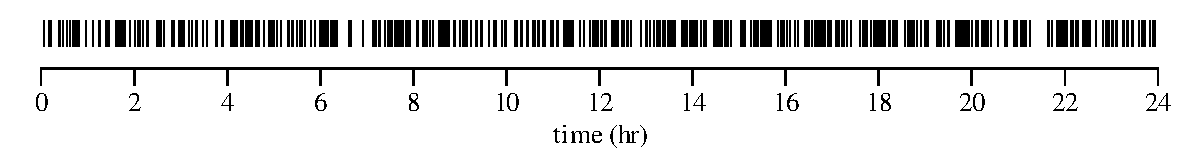
\includegraphics[width=\linewidth]{../figures/quakerug.pdf}
\begingroup \captionof{figure}{The time of day for all 543 magnitude
  5.0 or greater earthquakes of Figure~\ref{fig:declusteredquakes}.}
\endgroup
  
\end{itemize}

We will not discuss these, or most other distributions, in any detail.
Instead, we will focus our attention on one distribution, the Gaussian
distribution, which is so common that it is also known as the
\textbf{normal} distribution, implying that all other distributions
are `abnormal'.

\section{The Central Limit Theorem}
\label{sec:CLT}

Let us revisit the Old Faithful dataset of Figure~\ref{fig:KDE2D}.
  
\noindent\begin{minipage}[t][][b]{.35\textwidth}
  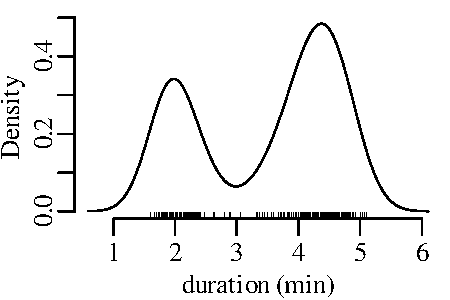
\includegraphics[width=\textwidth]{../figures/CLTfaithful1.pdf}\medskip
\end{minipage}
\begin{minipage}[t][][t]{.65\textwidth}
  \captionof{figure}{The KDE and rug plot of 272 Old Faithful eruption
    durations is the marginal distribution of
    Figure~\ref{fig:KDE2D}. This distribution has two modes at 2 and
    4.5 minutes.}
  \label{fig:CLTfaithful1}
\end{minipage}

The next three figures derive three new distributions by taking the
sum of $n$ randomly selected values from the geyser eruption
durations:

\noindent\begin{minipage}[t][][b]{.35\textwidth}
  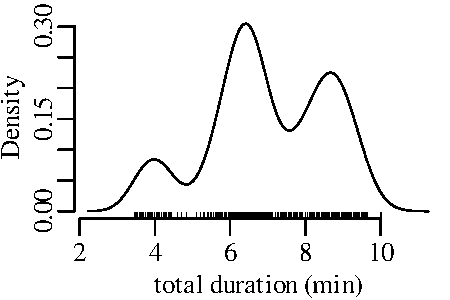
\includegraphics[width=\textwidth]{../figures/CLTfaithful2.pdf}\medskip
\end{minipage}
\begin{minipage}[t][][t]{.65\textwidth}
  \captionof{figure}{Collect $n=2$ randomly chosen events from the
    original dasaset of geyser eruptions with replacement and add
    their durations together. Repeat to create a new dataset of
    $N=500$ values.  The KDE of this distribution has not two but
    three modes at 4 ($=2\times{2}$), 6.5 ($=2+4.5$), and 9
    ($=2\times{4.5}$) minutes, respectively.}
  \label{fig:CLTfaithful2}
\end{minipage}

\noindent\begin{minipage}[t][][b]{.35\textwidth}
  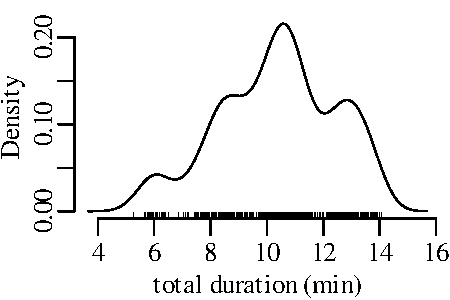
\includegraphics[width=\textwidth]{../figures/CLTfaithful3.pdf}\medskip
\end{minipage}
\begin{minipage}[t][][t]{.65\textwidth}
  \captionof{figure}{Collect $n=3$ randomly chosen events from the
    geyser eruption dataset and add their durations together. Repeat
    $N=500$ times to create a third dataset.  The KDE of this
    distribution has four visible modes, including peaks at 6
    ($=3\times{2}$), 8.5 ($=2\times{2}+4.5$), 11 ($=2+2\times{4.5}$)
    and 13.5 ($=3\times{4.5}$) minutes. }
  \label{fig:CLTfaithful3}
\end{minipage}

\noindent\begin{minipage}[t][][b]{.35\textwidth}
  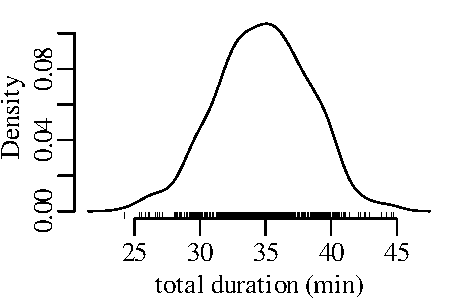
\includegraphics[width=\textwidth]{../figures/CLTfaithful10.pdf}\medskip
\end{minipage}
\begin{minipage}[t][][t]{.65\textwidth}
  \captionof{figure}{Taking $N=500$ samples of $n=10$ randomly
    selected eruptions and summing their durations produces a fourth
    dataset whose KDE has a single mode with symmetric tails towards
    lower and higher values.}
  \label{fig:CLTfaithful10}
\end{minipage}

Figure~\ref{fig:CLTfaithful10} has the characteristic \emph{bell
  shape} of a Gaussian distribution, which is described by the
following PDF:
\begin{equation}
  f(x|\mu,\sigma) = \frac{1}{\sigma\sqrt{2\pi}}
  \exp\!\left[-\frac{(x-\mu)^2}{2\sigma^2}\right]
  \label{eq:gauss}
\end{equation}

\noindent where $\mu$ is the \textbf{mean} and $\sigma$ is the
\textbf{standard deviation}. It can be mathematically proven that the
\emph{sum} of $n$ randomly selected values converges to a Gaussian
distribution, provided that $n$ is large enough. This convergence is
guaranteed \textit{regardless of the distribution of the original
  data}.  This mathematical law is called the \textbf{Central Limit
  Theorem}.\medskip

The Gaussian distribution is known as the normal distribution because
it naturally arises from \emph{additive processes}, which are very
common in nature. It is easy to create normally distributed values in
a laboratory environment. There even exists a machine that generates
normally distributed numbers:

\noindent\begin{minipage}[t][][b]{.55\textwidth}
  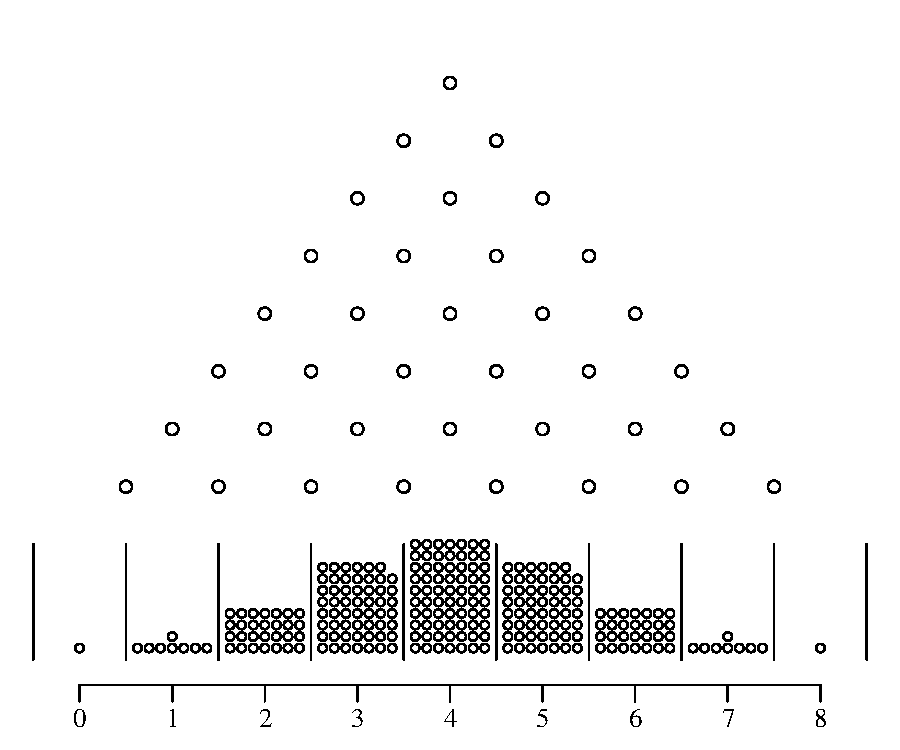
\includegraphics[width=\textwidth]{../figures/galtonsbeanmachine.pdf}\medskip
\end{minipage}
\begin{minipage}[t][][t]{.45\textwidth}
  \captionof{figure}{Galton's bean machine is a mechanical device that
    simulates additive physical processes. It consists of a triangular
    arrangement of pegs above a linear array of containers.  When a
    bead enters the machine from the top, it bounces off the pegs on
    its way down to the containers. The probability of bouncing to the
    left is the same as the probability of bouncing to the
    right. After $n$ bounces, the bead lands in one of the containers,
    forming a bell shaped (binomial) distribution. With increasing
    $n$, this distribution converges to a Gaussian form.}
  \label{fig:galtonsbeanmachine}
\end{minipage}

Additive processes are very common in physics. For example, when a
drop of ink disperses in a volume of water, the ink molecules spread
by colliding with the water molecules.  This \emph{Brownian motion}
creates a Gaussian distribution, in which most ink molecules remain
near the original location ($\mu$), with wide tails in other
directions.

\section{The multivariate normal distribution}
\label{sec:multinorm}

The binomial, Poisson, negative binomial, multinomial, uniform and
univariate normal distributions are but a small selection from an
infinite space of probability distributions. These particular
distributions were given a specific name because they commonly occur
in nature.  However the majority of probability distributions do not
fall into a specific parametric category.  For example, the bivariate
distribution of Old Faithful eruption gaps and durations
(Figure~\ref{fig:KDE2D}) is not really captured by any of the
aforementioned distributions. In fact, it is quite easy to invent
one's own distributions. Here are four examples of such creations in
two-dimensional data space:\medskip

\noindent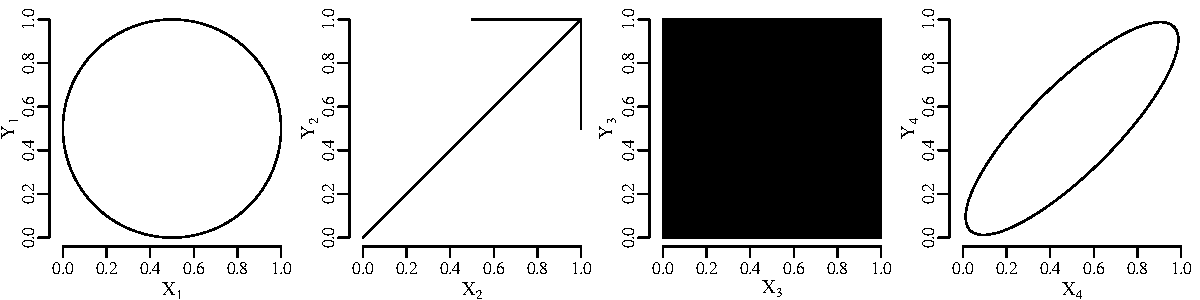
\includegraphics[width=\textwidth]{../figures/pop2d.pdf}
\begingroup \captionof{figure}{Four synthetic bivariate continuous
  distributions, defined by black areas and lines. White areas are
  excluded from the distributions.\medskip}
\label{fig:pop2d}
\endgroup

Let us collect $n=100$ random $(X,Y)$ samples from these four
distributions and plot them as four scatter plots:\medskip

\noindent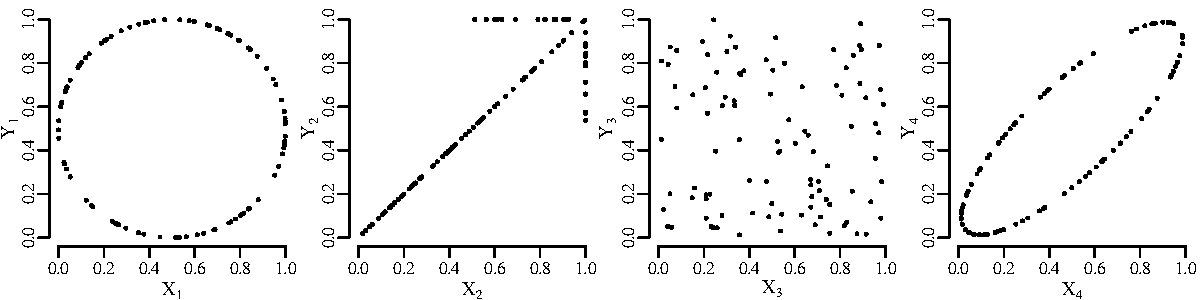
\includegraphics[width=\textwidth]{../figures/rand2d.pdf}
\begingroup \captionof{figure}{It is easy to recognise the probability
  distributions of Figure~\ref{fig:pop2d} in the scatter plots of
  $n=100$ random points selected from them.\medskip}
\label{fig:rand2d}
\endgroup

Next, we can calculate the sum of all the sampled points in each of
the four panels in Figure~\ref{fig:rand2d}. This gives rise to four
new pairs of coordinates. Repeating this experiment $N=200$ times and
plotting the four resulting datasets as scatter plots:\medskip

\noindent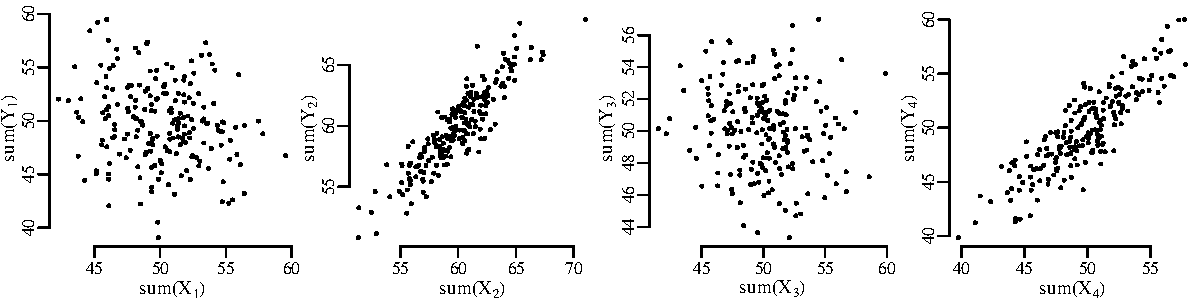
\includegraphics[width=\textwidth]{../figures/rand2dsum.pdf}
\begingroup \captionof{figure}{Four scatter plots with $N=200$ points,
  each of which represents the sum of a random sample of $n=100$
  points drawn from Figure~\ref{fig:pop2d}.\medskip}
\label{fig:rand2sum}
\endgroup

Despite the completely different appearance of the four parent
distributions (Figure~\ref{fig:pop2d}) and samples
(Figure~\ref{fig:rand2d}), the distributions of their sums
(Figure~\ref{fig:rand2sum}) all look very similar. They consist of an
elliptical point cloud that is dense in the middle and thins out
towards the edges. The density of the points per unit area is
accurately described by a bivariate Gaussian distribution:
\begin{equation}
f(x,y|\mu_x,\mu_y,\sigma_x,\sigma_y,\sigma_{x,y}) = \frac{
\exp\left(-
\left[\begin{array}{@{}cc@{}}
(x-\mu_x) & (y-\mu_y)
\end{array}\right]
\left[\begin{array}{@{}c@{}c@{}}
\sigma^2_x & \sigma_{x,y}\\
\sigma_{x,y} & \sigma^2_y
\end{array}\right]^{-1}
\left[\begin{array}{@{}c@{}}
x-\mu_x\\
y-\mu_y
\end{array}\right] \biggl/ 2
\right)
}{2\pi\sqrt{
\left|\begin{array}{@{}c@{}c@{}}
\sigma^2_x & \sigma_{x,y}\\
\sigma_{x,y} & \sigma^2_y
\end{array}\right|
}}
\label{eq:2dgauss}
\end{equation}

This matrix expression is completely described by five parameters: the
means $\mu_x$ and $\mu_y$, the standard deviations $\sigma_x$ and
$\sigma_y$, and the covariance $\sigma_{x,y}$. One-dimensional
projections of the data on the X- and Y-axis yield two univariate
Gaussian distributions.

\noindent\begin{minipage}[t][][b]{.45\textwidth}
  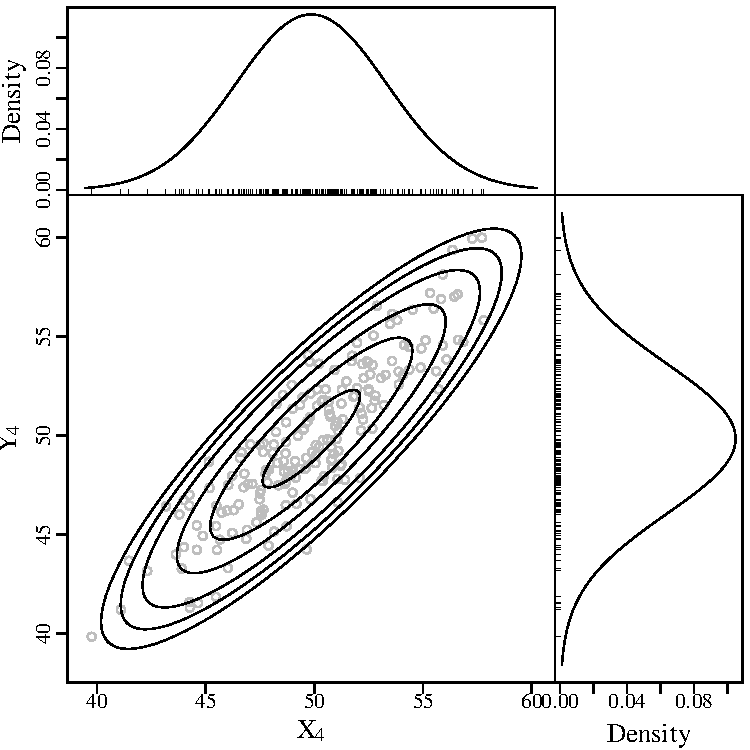
\includegraphics[width=\textwidth]{../figures/norm2dmarginal.pdf}\medskip
\end{minipage}
\begin{minipage}[t][][t]{.55\textwidth}
  \captionof{figure}{The main panel shows population 4 of
    Figure~\ref{fig:rand2sum} as grey circles, and the best fitting
    bivariate Gaussian distribution as contours. The side panels show
    the marginal distributions of the $X$- and $Y$-variable, which are
    both univariate Gaussian. The means and standard deviations of the
    marginal distributions equal the means and the standard deviations
    of the bivariate distribution. The bivariate distribution has a
    fifth parameter, the covariance $\sigma_{x,y}$, which controls the
    angle at which the elliptical contours are rotated relative to the
    axes of the diagram. The significance of these parameters is
    further explored in Section~\ref{sec:normalproperties}.}
  \label{fig:norm2dmarginal}
\end{minipage}

\section{Properties}
\label{sec:normalproperties}

The univariate normal distribution is completely controlled by two
parameters:

\begin{enumerate}
\item The \textbf{mean} $\mu$ controls the \textbf{location} of the
  distribution.  Because the normal distribution is unimodal and
  symmetric, the mean also equals the median and the mode.
\item The \textbf{standard deviation} $\sigma$ quantifies the
  \textbf{dispersion} of the distribution.
\end{enumerate}

\noindent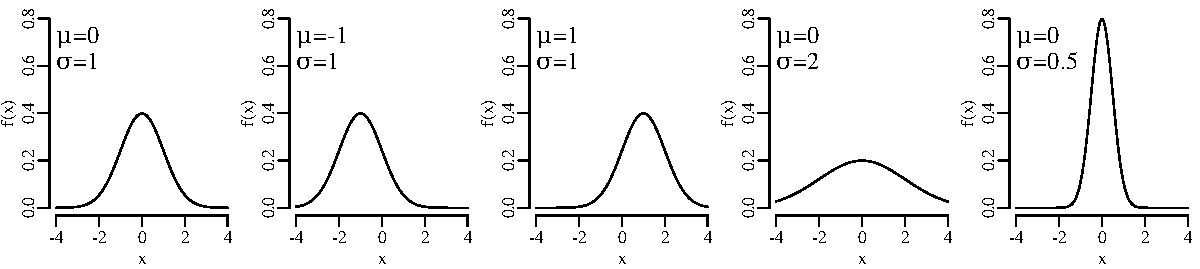
\includegraphics[width=\textwidth]{../figures/musigma.pdf}
\begingroup \captionof{figure}{PDFs of the univariate normal
  distribution for different values of $\mu$ and $\sigma$. $\mu$
  controls the position and $\sigma$ the width of the distribution. By
  definition, the area under the PDF always remains the same
  (i.e. $\int_{-\infty}^{+\infty}f(x)~dx = 1$).\medskip}
\label{fig:musigma}
\endgroup

The interval from $\mu-\sigma$ to $\mu+\sigma$ covers 68.27\% of the
area under the PDF, and the interval from $\mu-2\sigma$ to
$\mu+2\sigma$ covers 95.45\%. Conversely 95\% of the area under the
normal PDF is contained within an interval of $\mu\pm{1.96}\sigma$.

\noindent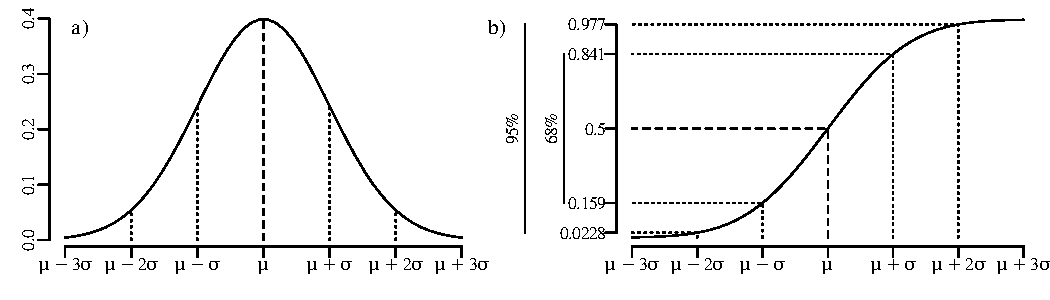
\includegraphics[width=\textwidth]{../figures/2sigma.pdf}
\begingroup \captionof{figure}{PDF (a) and CDF (b) of the normal
  distribution.  The $\mu\pm\sigma$ and $\mu\pm{2}\sigma$ intervals
  cover $\sim$68\% and $\sim$95\% of the distribution, respectively. }
\label{fig:2sigma}
\endgroup

\begin{enumerate}
  \setcounter{enumi}{2}
\item The \textbf{covariance} $\sigma_{x,y}$ controls the degree of
  \textbf{correlation} between two variables ($x,y$) in a bivariate
  normal distribution.
\end{enumerate}

\noindent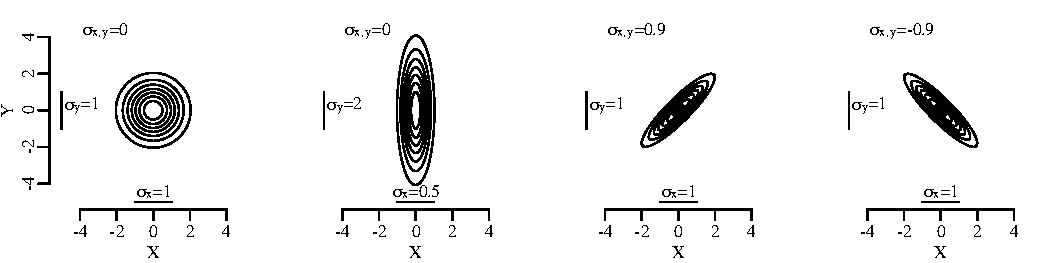
\includegraphics[width=\textwidth]{../figures/cov.pdf}
\begingroup \captionof{figure}{The standard deviations $\sigma_x$ and
  $\sigma_y$, and covariance $\sigma_{x,y}$ control the shape and
  dispersion of the bivariate normal distribution.\medskip}
\label{fig:cov}
\endgroup

The 1$\sigma$ contour around the mean of a bivariate normal
distribution only covers 39\% of the probability instead of $68\%$ for
the univariate normal distribution, and the 2$\sigma$ interval covers
86\% of the probability instead of the 95\% of the univariate
distribution.

\section{Parameter estimation}
\label{sec:normalparameters}

$\mu$ and $\sigma$ are \emph{unknown} but can be \emph{estimated} from
the data. Just like the binomial parameter $p$
(Section~\ref{sec:binompar}) and the Poisson parameter $\lambda$
(Section~\ref{sec:poispar}), this can be done using the method of
maximum likelihood.  Given $n$ data points $\{x_1, x_2, \ldots,
x_n\}$, and using the multiplication rule, we can formulate the normal
likelihood function as
\begin{equation}
  \mathcal{L}(\mu,\sigma|x_1,x_2,\ldots,x_n) =
  \prod\limits_{i=1}^{n}f(x_i|\mu,\sigma)
  \label{eq:Lnorm}
\end{equation}

$\mu$ and $\sigma$ can be estimated by maximising the likelihood or,
equivalently, the log-likelihood:
\begin{equation}
  \begin{split}
    \mathcal{LL}(\mu,\sigma|x_1,x_2,\ldots,x_n) & =
    \sum\limits_{i=1}^{n}\ln\left[f(x_i|\mu,\sigma)\right] \\ & =
    \sum\limits_{i=1}^{n} -\ln[\sigma] - \frac{1}{2}\ln[2\pi] -
    \frac{(x_i-\mu)^2}{2\sigma^2}
  \end{split}
  \label{eq:LLnorm}
\end{equation}

Taking the derivative of $\mathcal{LL}$ with respect to $\mu$ and
setting it to zero:
\begin{equation}
  \begin{split}
    \left.\frac{\partial{\mathcal{LL}}}{\partial{\mu}}\right|_{\hat{\mu}} & =
    - \sum\limits_{i=1}^{n} \frac{x_i-\hat{\mu}}{\sigma^2} = 0 \\
    & \Rightarrow n\hat{\mu} - \sum\limits_{i=1}^{n} x_i = 0 \\
    & \Rightarrow \hat{\mu} = \frac{1}{n}\sum\limits_{i=1}^{n}x_i
  \end{split}
\end{equation}

\noindent which is the same as Equation~\ref{eq:mean}. Using the same
strategy to estimate $\sigma$:
\begin{equation}
  \label{eq:stdevgivenmu}
  \begin{split}
    \left.\frac{\partial{\mathcal{LL}}}{\partial{\sigma}}\right|_{\hat{\sigma}}
    & = \sum\limits_{i=1}^{n} - \frac{1}{\hat{\sigma}} +
    \frac{(x_i-\mu)^2}{\hat{\sigma}^3} = 0\\
    & \Rightarrow  \sum\limits_{i=1}^{n} \frac{(x_i-\mu)^2}{\hat{\sigma}^3} =
    \frac{n}{\hat{\sigma}} \\
    & \Rightarrow \hat{\sigma} =
    \sqrt{\frac{1}{n}\sum\limits_{i=1}^{n}(x_i-\mu)^2}\\
  \end{split}
\end{equation}

\noindent which is \emph{almost} the same as the formula for the
standard deviation that we saw in Section~\ref{sec:dispersion}
(Equation~\ref{eq:stdev}):
\begin{equation}
  s[x] = \sqrt{\frac{1}{n-1}\sum\limits_{i=1}^{n}(x_i-\bar{x})^2}
  \label{eq:stdevrepeat}
\end{equation}

There are just two differences between
Equations~\ref{eq:stdev}/\ref{eq:stdevrepeat} and
Equation~\ref{eq:stdevgivenmu}:
\begin{enumerate}
\item Equation~\ref{eq:stdevgivenmu} uses the population mean $\mu$,
  whereas Equation~\ref{eq:stdev} uses the sample mean $\bar{x}$.
\item Equation~\ref{eq:stdevgivenmu} divides the sum of the squared
  differences between the measurements and the mean by $n$, whereas
  Equation~\ref{eq:stdev} divides it by ($n-1$).
\end{enumerate}

The two differences are related to each other. The subtraction of 1
from $n$ is called the \textbf{Bessel correction} and accounts for the
fact that by using an estimate of the mean ($\bar{x}$), rather than
the true value of the mean ($\mu$), we introduce an additional source
of uncertainty in the estimate of the standard deviation. This
additional uncertainty is accounted for by subtracting one
\textbf{degree of freedom} from the model fit.\medskip

Finally, for multivariate normal datasets, we can show that (proof
omitted):
\begin{equation}
  \hat{\sigma}_{x,y} = \sum\limits_{i=1}^{n}\frac{1}{n}(x_i-\mu_x)(y_i-\mu_y)
\end{equation}

\noindent or, if $\mu_x$ and $\mu_y$ are unknown and must be estimated
from the data as well:
\begin{equation}
  s[x,y] = \sum\limits_{i=1}^{n}\frac{1}{n-1}(x_i-\bar{x})(y_i-\bar{y})
  \label{eq:sxy}
\end{equation}

